\printMiniToc



\begin{note}
	Dans cette partie, j'expliquerai les détails de l'univers que j'ai créé pour ce jeu ainsi que les raisons qui m'ont poussé à faire les choix menant à cette fiction. L'univers n'est cependant pas terminé; s'il suffit largement aux besoins du jeu, il pourrait, dans l'optique de la réalisation d'une version complète, être agrandi et complété. De plus, certains détails, exprimés dans ce texte, dépassent déjà la portée de la démo.
\end{note}



\section*{Les thèmes importants pour le jeu}
Comme je l'ai déjà indiqué dans la section \ref{sec:objectifsTM}, ce jeu est l'occasion pour moi de développer des thématiques qui me semblent importantes. C'est un jeu d'opinion qui se veut le défenseur de mes points de vue.

Le thème le plus important est la relation humaine à la Nature. J'ai toujours été fasciné par la beauté de cette dernière, sa cruauté, à la fois son ordre parfait et son désordre total. Pour moi, un retour à la Nature est une condition nécessaire pour atteindre le bonheur. La relation que nous entretenons avec elle, collaborative ou dominante, sera donc au c\oe ur du jeu et ce choix déterminera de nombreux aspects de l'histoire et du gameplay\definition.

Il existe cependant de multiples contradictions entre ma passion pour la Nature et l'univers qui m'entoure. Comment ne pas constater les dégâts que nous infligeons à notre environnement? Mais plus encore, comment ne pas constater que notre mode de vie (que certains nomment consumérisme) a perdu toute sa simplicité, son sens, sa \enquote{naturalité}. Ce jeu sera donc l'occasion de mettre le doigt sur ces paradoxes et l'opportunité de se poser certaines questions sur nos façons de faire.

Un autre thème conducteur sera la relation fraternelle (sororale dans le cas du jeu); sujet important à mes yeux, étant donné que j'ai moi-même un frère. Le jeu gravitera aussi autour de la question de l'utilisation bénéfique et responsable ou destructrice et irresponsable de la technologie, des améliorations qu'elle peut apporter ou des dommages qu'elle peut causer et des abus auxquels elle peut conduire. Finalement, la question de la religion sera abordée, bien que dans une moindre mesure: quelle utilité a-t-elle? à quelles dérives peut-elle mener?


\section{Un monde divisé entre deux peuples}
Le jeu se déroule dans un univers, nommé \nomUnivers, qui est principalement divisé entre deux peuples: les Humains et les \nomNaturels s.

Les Humains sont une faction terne, grise et soumise à un tyran: Lord Gaamon. Le despote, atteint de folie, a une peur viscérale de la Nature et a convaincu le reste de la population de sa nocivité. L'utilisation de technologies mécaniques, polluantes et parfois brutales est monnaie courante et permet aux hommes de dominer les autres peuples habitant \nomUnivers; mais cela ne peut se faire sans ravager l'environnement. Ce peuple perdu et sombrant dans la peur a, pour sa plus grande majorité, oublié son histoire et exécute les ordres de Gaamon sans sourciller. Mais si certains hommes se laissent aller à la violence ou l'obéissance, d'autres à l'inverse tentent de résister physiquement, ou mentalement du moins. Ce sont les \enquote{Naturels}, mais ils ne représentent qu'une petite minorité de la population totale. La population humaine vit enfermée dans \nomVille, une ville énorme, entourée de hautes murailles. Les Humains représentent un peuple perverti, apeuré et aveugle.

Les \nomNaturels s, à l'inverse des Hommes, représentent un peuple plus pacifique qui accorde beaucoup d'importance à la Nature et tente de vivre en accord avec elle. Le nom \enquote{\nomNaturels s} est une anagramme de \enquote{Naturels} et pourrait se rapporter à l'adjectif \enquote{tellurique} qui signifie \enquote{de la terre}. Ce peuple est cependant sur le déclin. Autrefois au sommet de son art, c'est maintenant une nation dont les fondations même s'effritent.


\section{Les Humains}

\subsection{L'histoire humaine en quelques mots}

\begin{note}
	Cette section décrit en quelques mots l'histoire des hommes. Certains détails supplémentaires sont décrits à la section \ref{sec:HistoireGaamon}.
\end{note}


20 ans avant le début du jeu, la ville n'était encore qu'un petit village agréable, nommé Murtos. La vie agricole, bien que rude et laborieuse, y était appréciée et rares étaient les histoires qui venaient troubler la quiétude des habitants. Mais tout cela changea le jour où le jeune Gaamon arriva...

L'étranger décida de s'installer dans le bourg et fonda, ce qui était alors une nouveauté, la première usine d'\nomUnivers. Son succès fut rapide: il apportait du travail et produisait beaucoup grâce aux machines qu'il construisait. Il agrandit bientôt son usine... puis en construisit une deuxième, qu'il agrandit aussi. Grâce à cela, les conditions de vie s'améliorèrent, tout le monde avait du travail et la population était heureuse de cette venue providentielle.

L'ambition de Gaamon étant véritablement grande, il fit construire d'autres usines, créa d'autres machines, employa bientôt tout le village et draina les populations des alentours dans ses halles de production. Les affaires allaient bon train, l'argent coulait à flots et son influence ne cessait de s'étendre.

\begin{wrapfigure}[11]{r}{.38\textwidth}
	\vspace*{-.8cm}
	\center
	\includegraphics[width=\linewidth]{images/Monde/drapeauGaamonLarge.png}
	\caption{Emblème de Gaamon}
\end{wrapfigure}

Avec les années, il fédéra tous les Humains sous la bannière unique de ses usines et devint le maître incontesté de ce qui était devenu une ville. Mais Gaamon n'était pas complètement sain d'esprit; cachée au fond de lui résidait une folie haineuse de la Nature. Le pouvoir et l'argent permirent à cette phobie, jusqu'alors refoulée, de s'exprimer de plus en plus pleinement et ouvertement. Il avait réussi à industrialiser, mécaniser le village, il voulait maintenant étendre son emprise hors des limites de la cité.

Il fortifia la ville en construisant des murailles et bâtit, en son centre, une immense tour d'acier et de verre qui devint l'icône emblématique de son empire. Il imposa à tous l'interdiction de sortir de l'enceinte des murs et brûla les dernières traces de verdure dans la cité. Il s'engagea alors, depuis le haut de sa nouvelle forteresse, dans un projet d'éradication plus vaste, qui annihilerait toute Nature, plantes ou animaux, des terres environnantes. Le jeu débute quelques années après le commencement de ce funeste projet, à l'intérieur de la ville.

\vspace*{-1mm}
\subsection{Petite biographie de Gaamon}
\begin{figure}[p]
	\center
	\thisfloatpagestyle{empty}
	
\includegraphics[width=\textwidth]{./images/Monde/Personnages/gaamonPortrait.png}
	\caption{Lord Gaamon\label{fig:Gaamon}}
\end{figure}

\vspace*{-2mm}
\descrPersoTitle[0]{Ses habits}
Gaamon est vétu d'une longue cape violette et d'un haut de forme masquant son visage par l'ombre qu'il créer. Il est aussi muni d'un \oe il mécanique rouge luisant (\textit{cf.} figure \ref{fig:Gaamon}).

\descrPersoTitle{Ses caractéristiques principales}
Il dirige la ville d'une main de fer depuis le haut de sa tour, il déteste la Nature au plus haut point et veut l'éradiquer par tous les moyens. Gaamon est doté d'une capacité innée à jouer avec les engrenages et les pistons; il a toujours eu un don pour la création de machines. Il en imaginera quantité; au départ pour aider dans ses usines, puis d'autres plus compliquées comme les Gnobols (\textit{cf.} section \ref{sec:Gnobols}) pour asseoir son empire.

\newpage
\descrPersoTitle{Son histoire}
\label{sec:HistoireGaamon}
\textbf{Adolescent}\quad Gaamon était un jeune homme plein de vie, d'enthousiasme et de bonne humeur. Son charisme indéniable semblait le promettre à un avenir radieux et, aimé de tous --- villageois comme camarades de jeu, il profitait innocemment de ce temps joyeux.

Mais lors de ce jour maintenant mille fois maudit par les dernières populations libres d'Éluria, il se perdit en forêt suite à un jeu avec ses amis. Il pénétra profondément dans ce lieu mystérieux avant de se rendre compte qu'il ne savait plus d'où il venait ni comment sortir. Seul et désemparé, il cria à l'aide, en vain, chercha, cria de nouveau, se mit à courir, mais la forêt se refermait sur lui, les branches lui griffaient le visage et les racines cherchaient à le faire trébucher. Il tenta de trouver la lisière et, ce faisant, ne s'enfonça que plus profondément dans cet univers à la fois plein d'enchantements et de maléfices. Son errance dura tant et si bien, qu'il finit par atteindre le c\oe ur même de la forêt, un lieu hautement sacré, réservé aux seuls esprits et rares élus, un lieu protégé par de multiples pièges et sortilèges afin d'en écarter les intrus.

Un de ces pièges se referma sur lui: il marcha sur un champignon empoisonné qui libéra brutalement ses spores vaporeux. Ces puissants psychotropes plongèrent le jeune homme dans un état de démence hallucinatoire très profonde. Il perdit toute conscience de la réalité et vécut l'horreur et la peur sous toutes leurs formes les plus profondes durant des heures, seul au c\oe ur de cet écrin terrifiant.

Personne ne sait comment, mais le garçon sortit de la forêt deux jours plus tard, ses vêtements en lambeaux, l'âme déchirée. Il lui fallut un peu plus de deux ans pour recouvrer la raison, mais jamais plus il ne fut le même. La vie perdit à ses yeux toute magie, devint terne et cruelle. Mais surtout, il emporta dès lors avec lui une peur absolue et une haine encore plus profonde de la Nature. Il restait un jeune homme beau, intelligent et malin mais il avait perdu l'espoir, la joie de vivre.

\textbf{Jeune adulte}\quad Quelques années plus tard, alors que le commerce de Gaamon à Murtos commençait à s'épanouir, il rencontra Miya; une jeune femme à la beauté exquise, particulièrement vive d'esprit, singulièrement perspicace et follement amoureuse de la vie, de sa simplicité et de sa beauté. Gaamon, immédiatement intrigué, voulu connaître cette personne si différente de lui et en même temps tellement séduisante. L'attraction fut réciproque et Miya fascinée, tant par la beauté ténébreuse que par l'esprit torturé mais néanmoins redoutable du jeune homme, fut pour ce dernier une lumière dans sa vie alors si sombre. Serait-elle celle qui lui permettrait de retrouver la joie de vivre?

Ils débutèrent une relation à la fois passionnée, fusionnelle et charnelle, vivant un bonheur profond et léger. Miya eut son premier enfant --- une magnifique fille --- au solstice d'été. Ils la nommèrent Lenaï comme l'héroïne d'un conte enfantin qu'ils affectionnaient tous les deux\footnote{Pour approfondir encore l'univers d'\nomUnivers, il pourrait être intéressant d'écrire un conte narrant l'histoire des Hommes et des Telurans au commencement de ce monde. Il pourrait avoir une signification particulière pour Gaamon et lui rendre un peu sa joie de vivre et son humanité quand il l'entend. Il pourrait être inséré dans le jeu comme une cinématique en images fixes (\textit{cf.} section \ref{sec:quatriemeActe} à ce sujet).}.

Le lien qui unissait les deux âmes éprises était très fort, particulièrement heureux et semblait augurer d'un avenir des plus brillants. Cependant, si Miya permettait au garçon de retrouver la joie de vivre, elle n'avait pas la capacité d'annuler sa haine pour la Nature. Et, les affaires de Gaamon, marchant bien, trop peut-être, lui permettaient d'assouvir ses volontés vengeresses. Il commença modestement et fit remplacer un parc par un immeuble, puis installa à l'emplacement de l'étang à la périphérie du village un centre d'épuration qui raya ce dernier de la carte. Ce fut ensuite au tour de la forêt avoisinante d'être rasée et remplacée par des usines. Au fil des mois, plus son influence grandissait, plus ses intentions devenaient évidentes.

Il fonda un parti --- le parti industrialiste --- qui rallia la majorité de la population, constatant bien que Gaamon apportait un confort de vie tout à fait révolutionnaire. Il cherchait principalement à rationaliser et améliorer les flux de production pour augmenter le bonheur général, mais ces idées étaient pour lui indissociables d'une haine destructrice contre la Nature. Un parti opposé vit le jour quasi simultanément, fondamentalement opposé aux idées du premier. Il prônait une idée de Nature et de paix, de simplicité et de bonheur. La guerre entre les deux fut immédiate. Toute proposition de l'un était immédiatement saluée par une contre-proposition de l'autre, contre chaque projet étaient déposées des motions, à chaque discours on constatait la présence d'opposants remontés.

Gaamon faisait tout son possible pour mettre des bâtons dans les roues de son adversaire politique, saper sa crédibilité et lier toujours plus de personnes à sa cause. À terme, sa stratégie eut les effets escomptés. Il réussit à discréditer les naturels et la plupart des habitants prirent fait et cause pour lui. Il leur avait apporté, à lui seul, confort, aisance et longévité.

Si le combat, au départ, était équilibré, la balance penchait soudain très fortement de son côté. Il se fit élire maire du village qui prenait de plus en plus l'apparence d'une ville et entreprit tout ce qu'il fallait pour réduire à néant le parti naturel. Interdiction de manifester, utilisation d'espions et d'agents doubles pour semer le trouble dans les rangs adverses, raids nocturnes pour apeurer les membres; toutes les stratégies étaient bonnes. L'interdiction totale du parti, finit de dissoudre l'entité politique et seul un groupuscule clandestin subsista.

Miya n'avait jamais senti le besoin de s'inscrire dans quelque combat politique que ce soit et se contentait de vivre heureuse dans le monde protégé et douillet qu'elle avait créé autour de son enfant. Elle profitait du temps qu'elle avait et suivait de loin les disputes incessantes sans pour autant y prendre part. Si elle devait appartenir à l'une des factions, ce serait celle des naturels; mais pourquoi faire? Quel intérêt y avait-il à prendre part à ce conflit, si ce n'était l'alimenter plus encore?

Petit à petit Gaamon pris le contrôle de la ville. Les conditions de vie changeaient, les murs des bâtiments s'élevaient toujours plus haut comme ceux d'une prison, les frontières avec la Nature étaient sans cesse repoussées et le tapis urbain semblait vouloir s'étendre sans fin pour former un entrelacs infini de routes et de bâtiments.

\textbf{Quelques années à peine plus tard}\quad Ces modifications amenèrent des tensions dans le couple; les disputes, jusque-là inexistantes, devinrent plus courantes. Miya ne pouvait comprendre la haine de son mari pour ce qu'elle considérait être une source vitale pour chaque homme. Elle ne pouvait cautionner la dynamique qu'il tentait d'instaurer. Elle ne pouvait supporter la façon dont les naturels avaient été réduits au silence. Mais c'est peut-être le contact sacré avec la Nature, maintenant réduit à néant, cette absence qu'elle n'avait jusque-là jamais vécue, qui lui lacérait le plus le c\oe ur; pourrait-elle vraiment élever sa fille, Lenaï, sans jamais lui montrer les arbres naissants au printemps, les fleurs chatoyantes d'été, la douce mélodie des oiseaux à la saison des amours ou le chant du ruisseau pur? Tout cela paraissait impossible. Alors Miya, horriblement partagée entre son amour et sa passion pour la Nature, prit une décision impossible; elle allait entrer dans les factions de la résistance naturelle.

Ce revirement, la jeune femme l'assuma pleinement et décida d'en faire un combat personnel. Elle s'attela à combattre les projets anti-naturels de Gaamon avec vigueur. Rapidement, l'acharnement, la rage et l'audace de Miya, portèrent la jeune femme au rang de légende dans le groupe secret. Elle prit la direction des rebelles et appliqua les principes mêmes de Gaamon: organisation, rationalisation, répartition. Elle affûta leur stratégie et aiguisa leur volonté, afin d'avoir une véritable armée sous ses ordres; et engagea une guerre de l'ombre terrible et destructrice contre le tyran, contre cette personnalisation de la haine de la Nature, contre son plus grand et seul amour.

Miya entretint dès lors une double-vie: elle était simultanément la femme ayant choisi de suivre amoureusement son mari et une furie s'acharnant contre tout ce qu'il entreprenait, la mère chérissant sa fille et la cheffe la plus virulente qu'aient pu avoir les guerriers naturels, l'ennemi juré sabotant les plans et l'être aimé attendant patiemment au lit le retour de sa moitié. Cette situation dichotomique torturait son âme atrocement. De jour, elle aimait Gaamon, son esprit puissant et sa volonté à toute épreuve, son aura mystérieuse et sa force. Parfois, la jeune mariée se surprenait même à penser que l'homme en face d'elle voulait le bien de la population et améliorait vraiment le niveau de vie. Mais de nuit, elle redevenait l'esprit acéré, tranchant qui trouvait la gloire parmi les rangs de l'ombre. Elle utilisait toutes les informations glanées durant la journée pour empêcher la volonté industrielle de s'accomplir. Elle était l'agent double le plus redoutable, le plus insoupçonnable et le plus déchiré. Ainsi, le couple dirigeant était aussi le couple divisant.

Gaamon, aveuglé par la révolte et la ténacité dont faisaient preuve les rebelles, bâtit à la gloire de sa puissance les murailles qui entourent encore aujourd'hui la ville afin de la \enquote{protéger de la Nature extérieure}. Les immenses portes blindées à l'est et à l'ouest de la ville, seuls points de passage, n'étaient encore fermées que la nuit.

C'est à ce moment que Miya commença à avoir des doutes quant au but qu'elle poursuivait. Elle avait perdu la joie de vivre. Elle n'avait pas vu la moindre pousse verte depuis des lustres. Elle se sentait perdue, son lien avec la Nature déchiré. Elle avait passé tellement de temps à se battre qu'elle en avait oublié pourquoi elle le faisait. Valait-il vraiment la peine de continuer ainsi, encore et encore? Cette escalade de violence conduirait-elle à une amélioration ou serait-elle la fondatrice d'un extrémisme renouvelé chez la population et son gouverneur? Mais la machine secrète était en marche et les naturels continuèrent, imperturbables, de perpétrer sabotages et destructions. 

La situation atteint un tel degré d'exacerbation que Gaamon, enragé par tous ces affronts, enflammé par toutes ces preuves que d'autres ne croyaient pas en sa vérité, la seule Vérité, décida de clore définitivement les portes de la Ville et déploya des escouades chargées de carboniser au lance-flamme les dernières traces de verdure.

Pour Miya, ce fut le signe indubitable qu'elle ne faisait qu'aggraver la situation; elle avait choisi la mauvaise méthode pour défendre sa cause! Elle se retira du groupuscule pour n'y plus revenir. Parmi les membres, cet acte fut perçu très différemment. C'était pour certains une marque de grande sagesse, pour d'autres la pire des trahisons, un abandon pur et simple.

Par une nuit sombre, l'un d'eux dénonça l'ex-leader à Gaamon, lui avoua l'ampleur de l'hypocrisie de sa femme qui, pendant tout ce temps, l'avait trompé. Miya, qui avait emmené Lenaï pour une balade ce soir-là, fût avertie par les partisans qui lui étaient restés fidèles que Gaamon avait lancé toutes les forces à sa disposition à sa recherche. Il était dans une rage absolument incroyable, personne ne l'avait jamais vu dans une fureur pareille. Miya n'avait d'autre solution que de fuir. Mais la ville était hermétiquement close. Impossible de quitter les lieux, il lui fallait se cacher. Cette nuit fut de pure horreur. Poursuivie, pourchassée, la jeune téméraire arpenta apeurée les rues désertées et sombres de Murtos. Mais vers qui se tourner? Si elle frappait à la mauvaise porte, elle ne manquerait pas de se faire dénoncer. Elle décida finalement de se cacher au fond de Redel, le quartier pauvre, là où la police n'osait pas s'aventurer. Elle savait qu'il y résidait un petit groupe de Naturels cachés, restés fidèles aux idéaux Telurans et qui n'avaient jamais accepté d'entrer dans le parti naturel de peur de participer à la dégradation de la situation. Ils avaient eu la sagesse qu'elle n'avait pas eue.

À son arrivée dans le quartier reculé, les habitants la dissimulèrent sans poser de question mais sans être totalement heureux de cette arrivée. Ils étaient chaleureusement distants à son égard. Mais ils semblaient avoir perdu, eux aussi, la joie de vivre.

Le deuxième enfant de Gaamon naquit quelques mois plus tard. Elle avait été conçue à peine quelques jours avant la fuite de Miya. La petite créature, babillarde et rose, fut nommée Kida, comme l'ancienne princesse Teluranne, glorieuse fondatrice de l'empire éponyme. Elle vécut son enfance avec son aînée, Lenaï, au c\oe ur de ce havre protégé, cette dernière perle agréable nichée au fond de l'écrin de dureté citadine qu'était le quartier des Naturels cachés de Redel.

\textbf{Quatorze ans plus tard}\quad Kida avait 14 ans quand sa mère, partie en ville pour acheter des provisions, se fit emprisonner par la garde de Gaamon; un ancien agent l'avait reconnue et dénoncée. Elle fut pendue publiquement le lendemain sur la place devant la Tour. Il est dit que le tyran, fou de colère, de rage et de haine, aurait torturé sa femme toute la nuit précédant la cérémonie dans les cachots sombres de son antre, l'aurait écouté lui raconter en détails chacune de ses trahisons pour le plaisir de souffrir et de la torturer, pour lui faire payer encore et encore et encore.



\begin{figure}[ht]
	\hspace*{-2cm}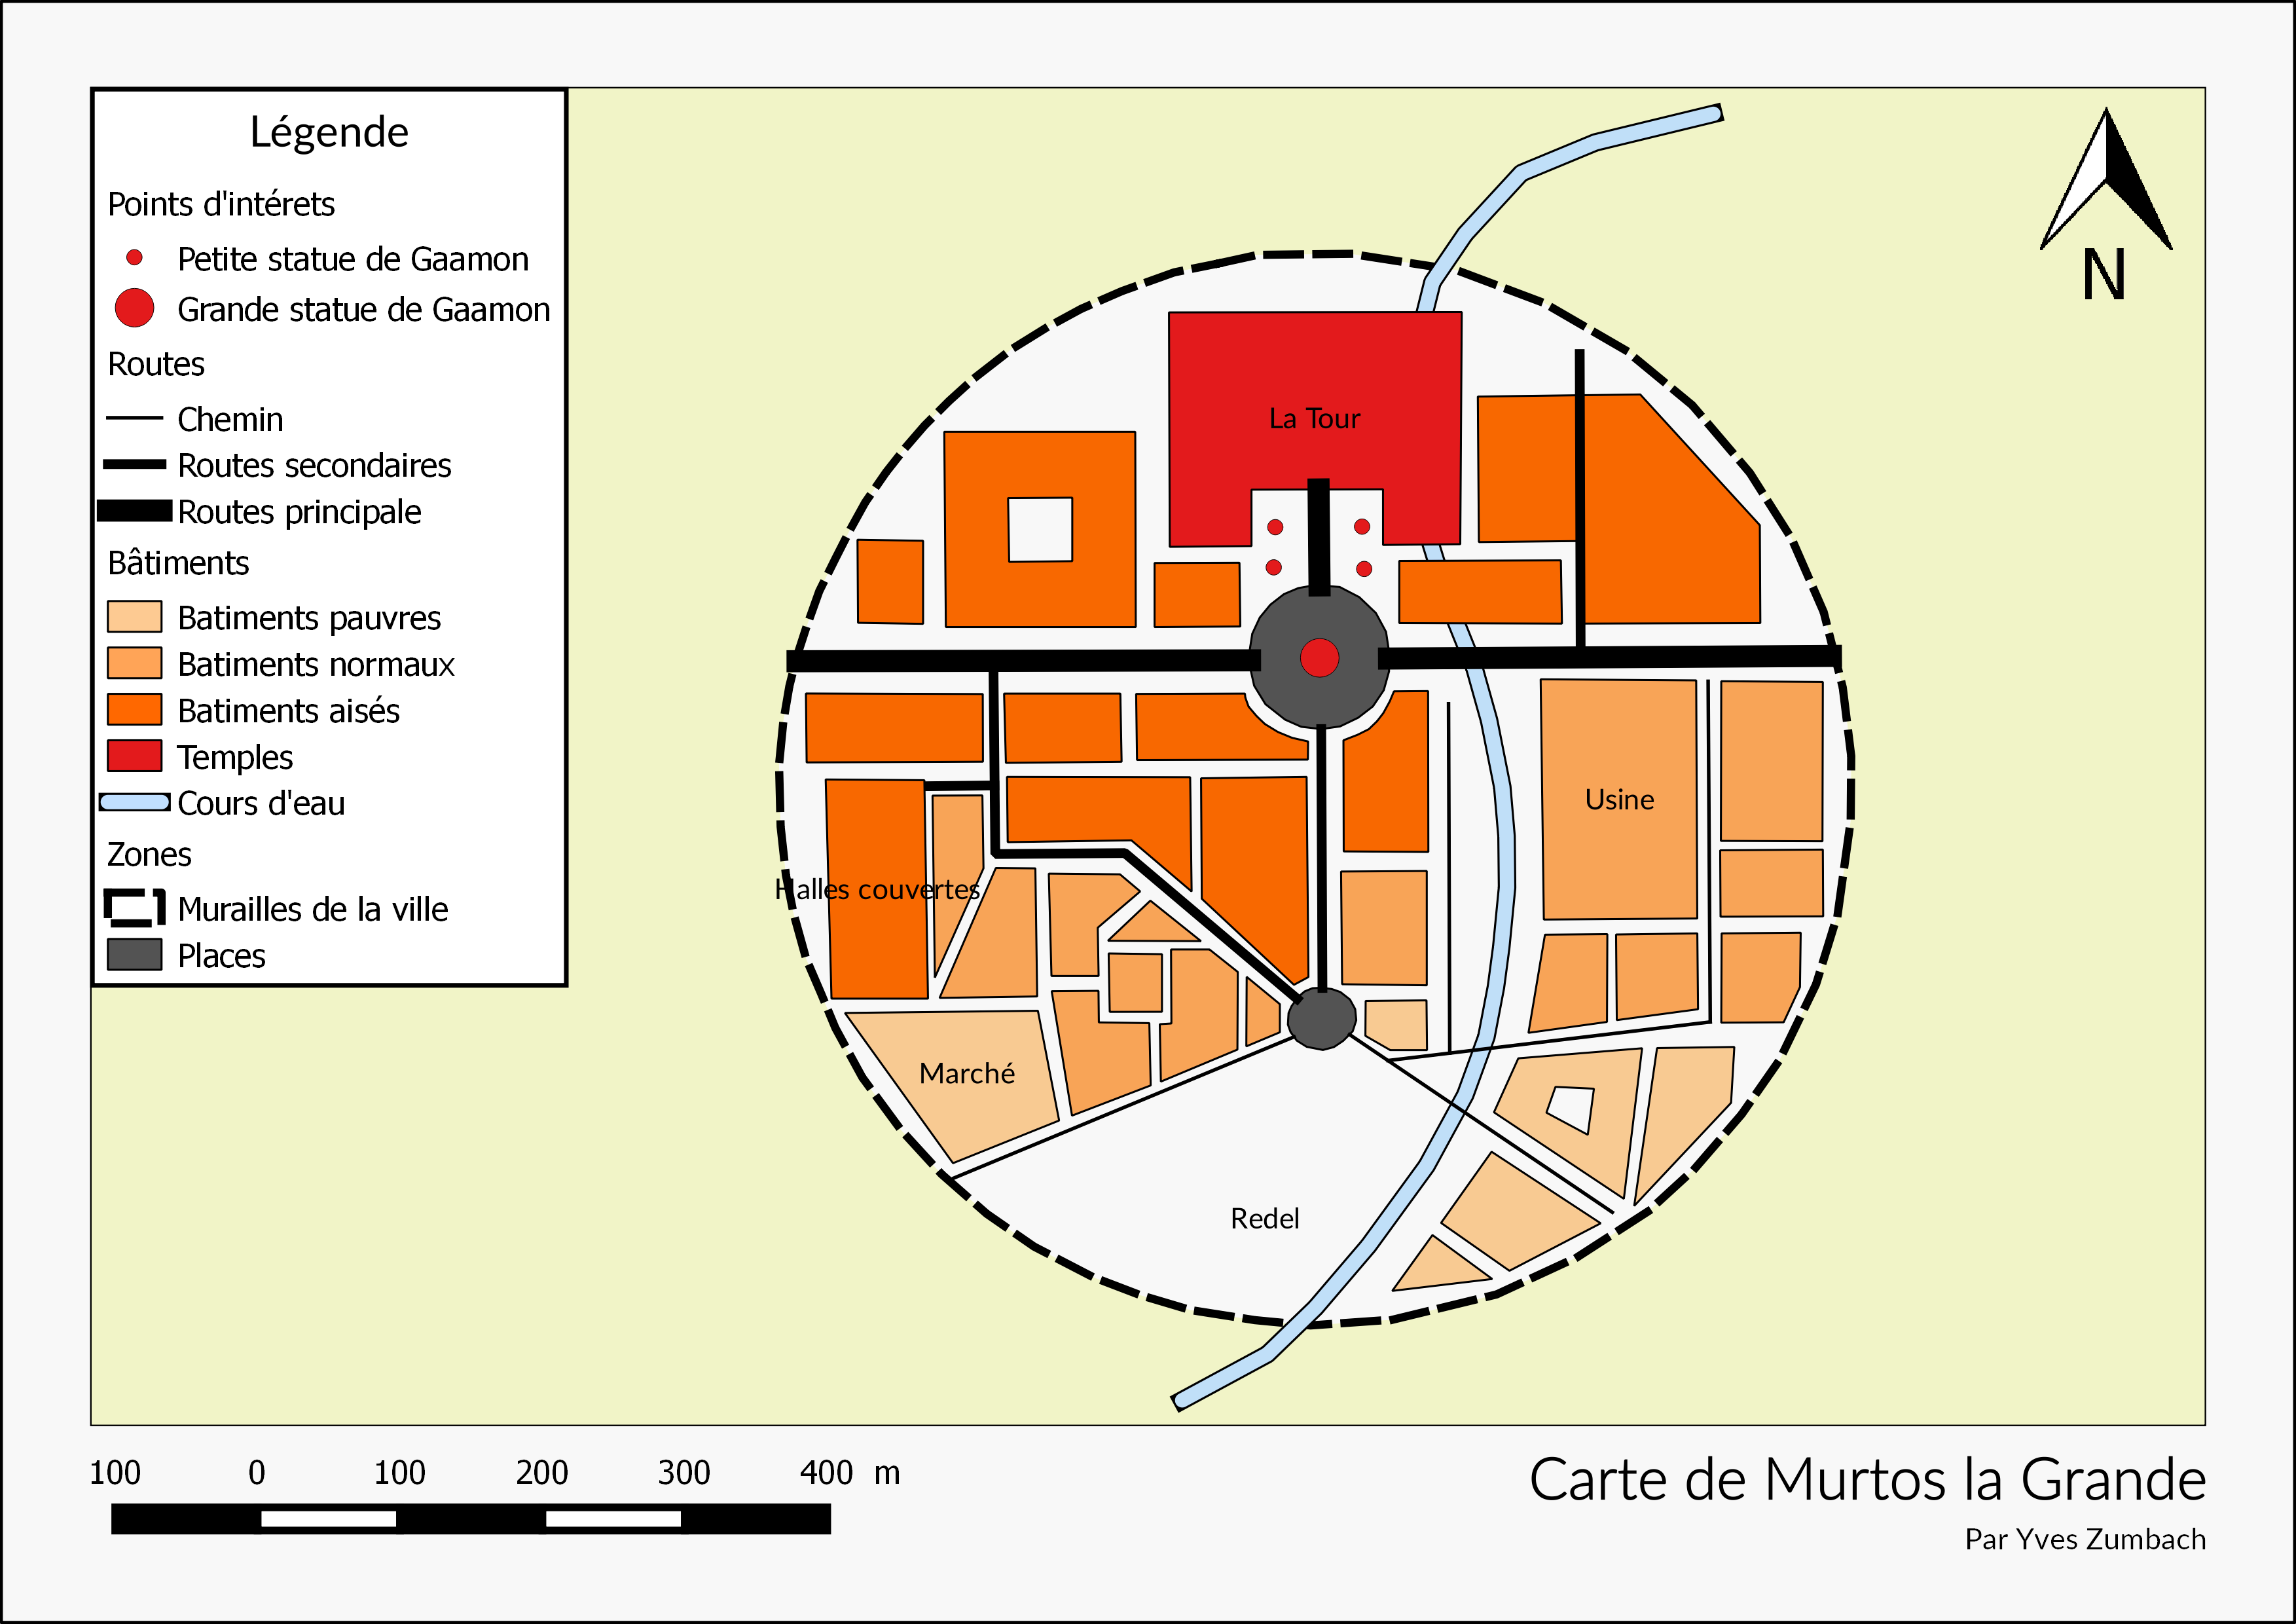
\includegraphics[width=\textwidth+2cm]{images/Monde/carteVille.png}
	\caption{Plan de Murtos la Grande (réalisé à l'aide du programme Quantum GIS)}
	\label{fig:murtosLaGrande}
\end{figure}

\subsection{La ville}
La ville est donc le bastion de la race humaine, l'empire de Lord Gaamon. Son décor relève de l'univers steampunk (\textit{cf.} annexe \ref{app:steampunk}). Il s'agit d'un monde urbain de l'ère industrielle où l'horizon est rythmé par les cheminées des hauts fourneaux qui crachent leurs fumées nauséabondes et où la suie recouvre les architectures de métal et de verre. Cet environnement, métaphoriquement, représente l'utilisation abusive de la technologie. C'est aussi la haine envers la Nature, sa négation totale. (plan de Murtos à la figure \ref{fig:murtosLaGrande})

\subsubsection{Redel, le quartier pauvre}
Les deux premiers niveaux du jeu (\textit{cf.} section \ref{sec:premierActe}) se déroulent dans le quartier pauvre, nommé Redel (\textit{cf.} cartes \ref{fig:murtosLaGrande} et \ref{fig:carteQuartierPauvre}). Il se situe à l'extrême sud de \nomVille. C'est le quartier le plus sale, où vivent les gens les plus pauvres.

Le coin sud-est du quartier est occupé par une énorme usine gouvernementale. L'accès à cette dernière est formellement interdit et des gardes surveillent en continu son entrée. De plus, elle crache sur le quartier des fumées toxiques, particulièrement malsaines à respirer.

\subsubsection{Un \enquote{bastion vert}}
Les dernières personnes à croire en la Nature habitent les maisons les plus isolées, au sud de Redel (\textit{cf.} carte \ref{fig:carteQuartierPauvre}). Ces gens cachent cependant leur croyance, de peur d'être persécutés. N'ayant plus vu une plante depuis des années, ils commencent à oublier ou à sombrer dans la superstition.

Un des trois sanctuaires de la Nature, celui de Tia, est caché dans ce quartier. Pour y accéder, un passage secret existe dans la maison située juste au nord de ce jardin caché. Cette dernière est habitée par Maïnin, un vieil homme sage qui a gardé l'esprit clair et lucide.


\subsection{Religion humaine}
La religion humaine est, à l'image de la ville, corrompue. Elle prône le bonheur par l'aisance matérielle, la richesse et la consommation. C'est même une apologie de la consommation --- si possible inutile --- que soutient ce dogme. De plus, les prêtres professent que l'argent ne s'acquiert que par le travail. Gaamon utilise la religion pour asservir les masses et motiver un travail acharné dans ses usines. Le symbole de ce culte possède une forme très caractéristique (\textit{cf.} figure \ref{subfig:accedeBonheur}) qui s'emboite avec l'icône de Gaamon pour représenter la collusion Religion--État. Quelques images de propagande que l'on peut trouver placardées sur les murs de la ville sont données à la figure \ref{fig:propagandeReligion}.

\vspace*{1cm}
\begin{figure}[ht]
	\subfloat[\label{subfig:accedeBonheur}Accède au Bonheur!]{
\includegraphics[width=.48\linewidth]{images/Monde/accedeAuBonheur.png}}
	\hspace*{.04\linewidth}\subfloat[Consommer pour la santé]{
\includegraphics[width=.48\linewidth]{images/Monde/consommerPourSante.png}}
	
	\subfloat[La Richesse c'est le Bonheur!]{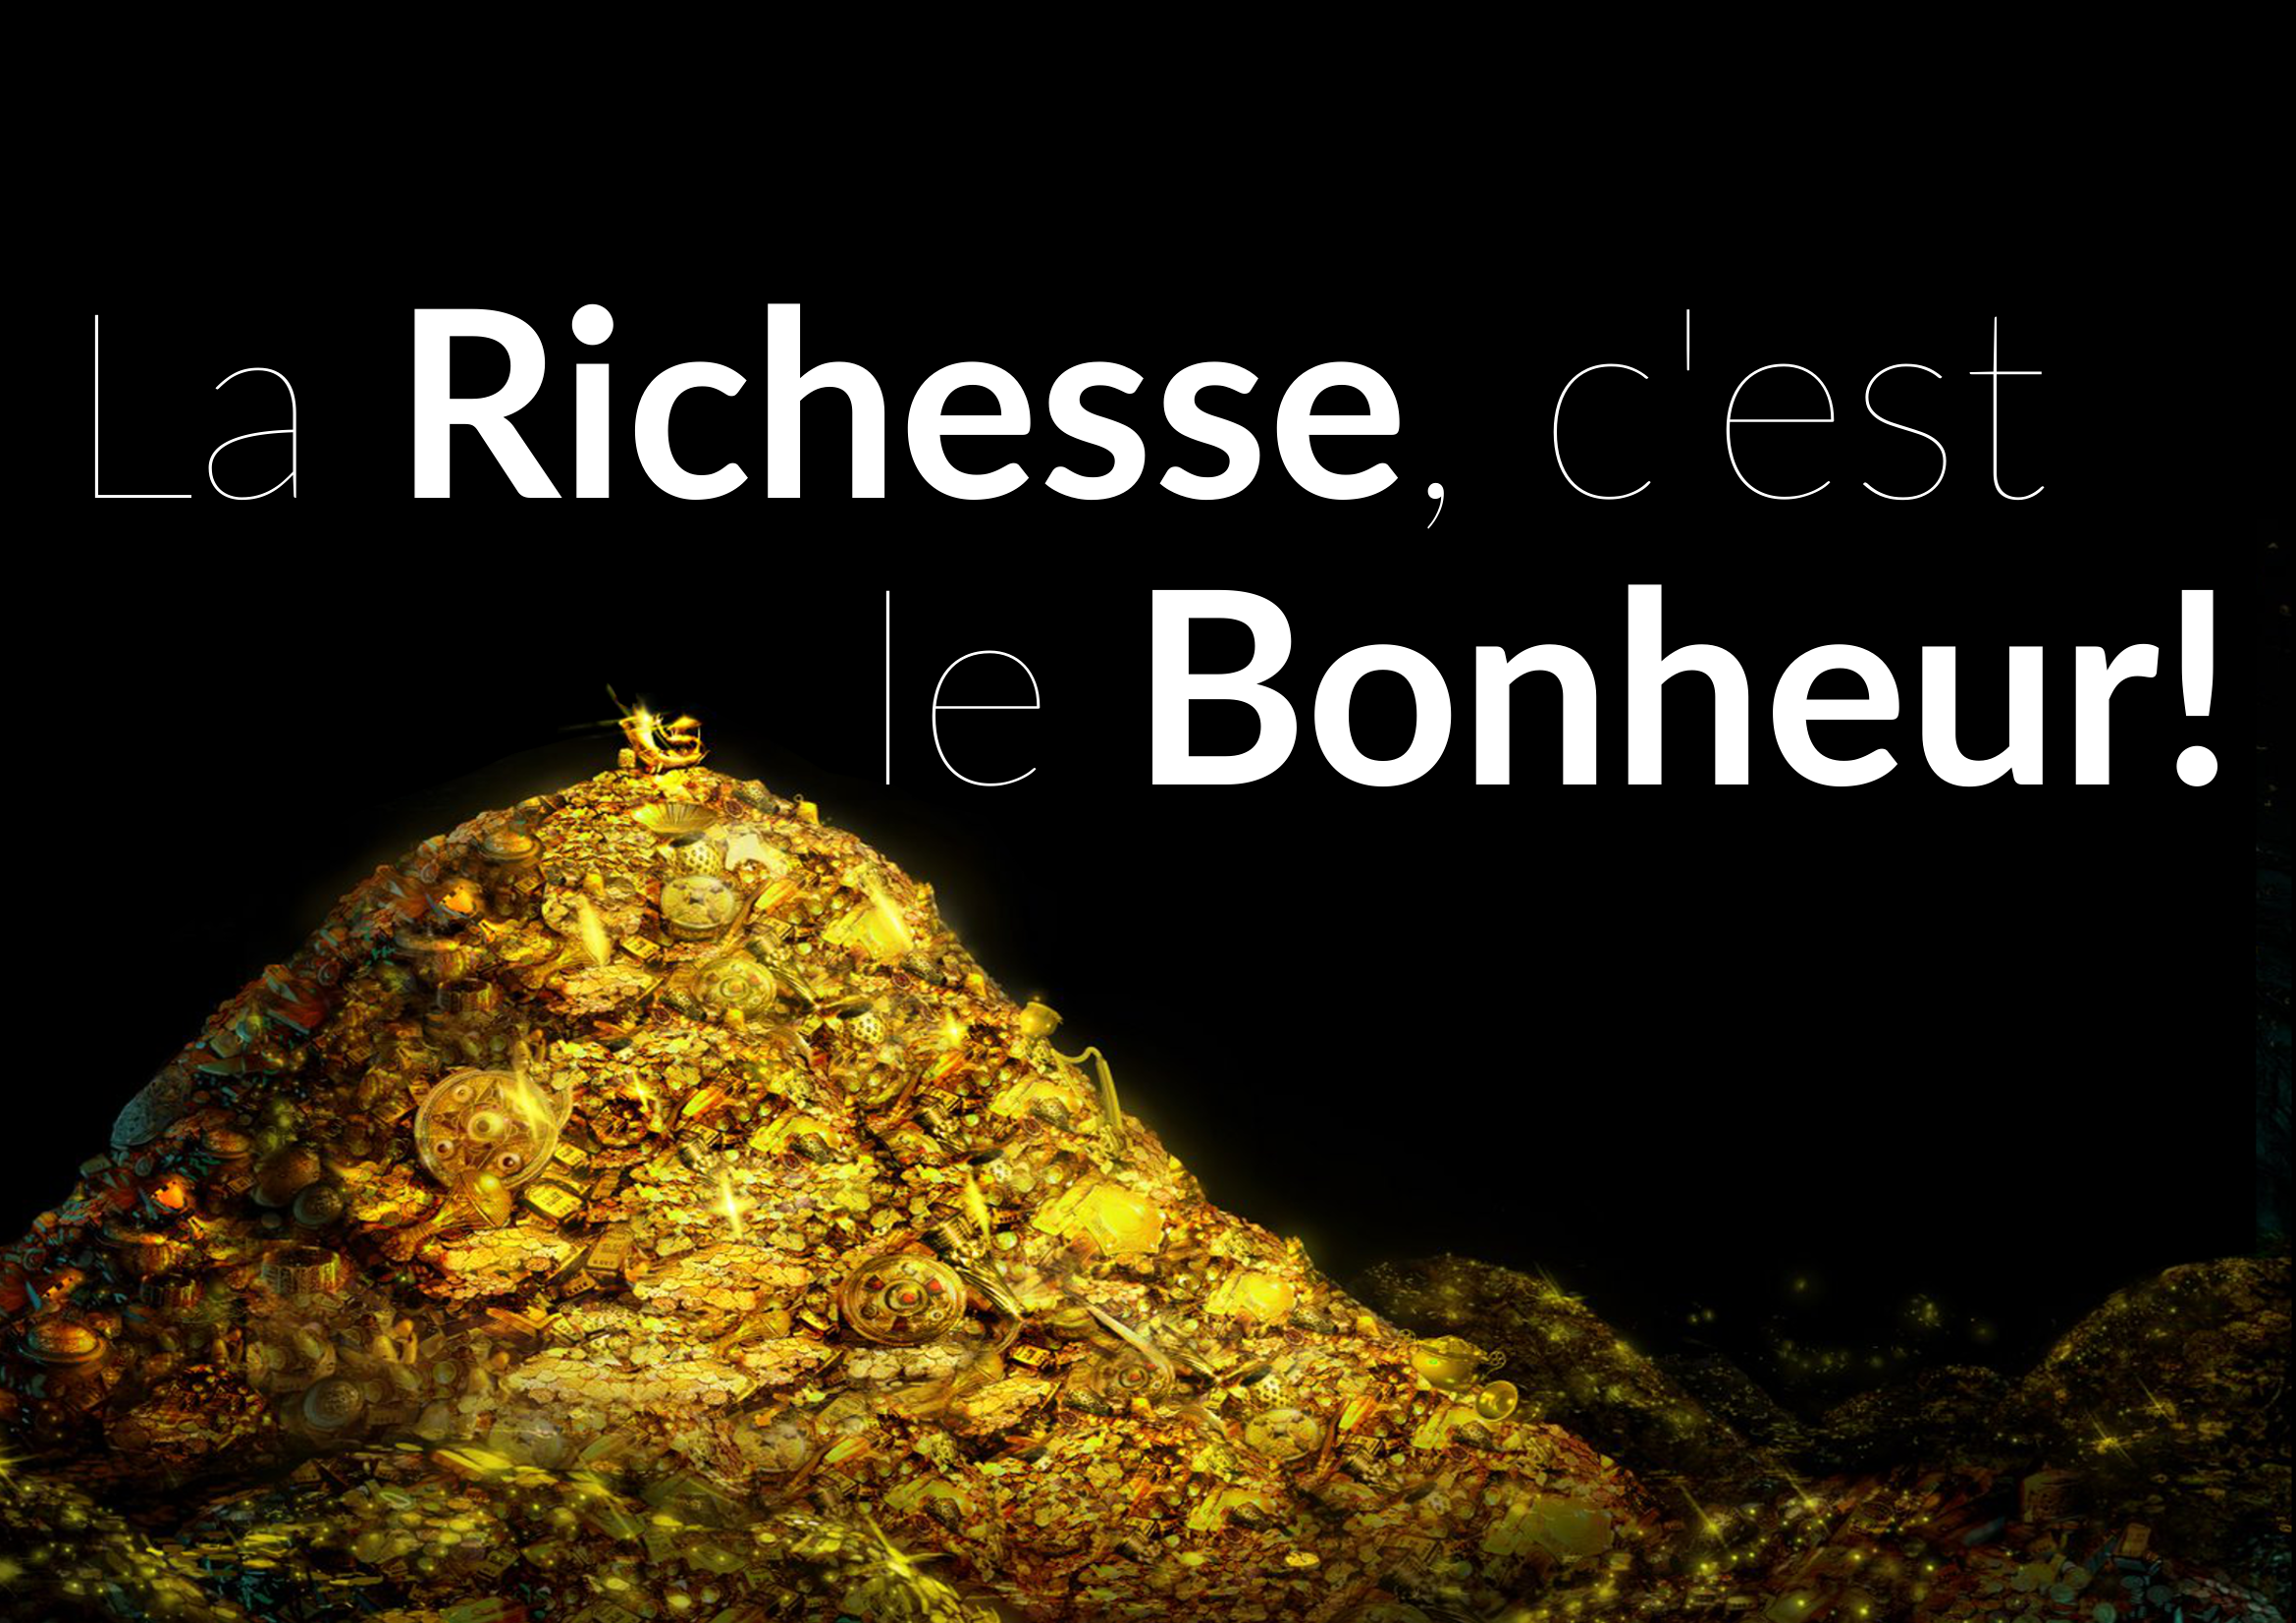
\includegraphics[width=.48\linewidth]{images/Monde/RichesseBonheur.png}}
	\hspace*{.04\linewidth}\subfloat[L'aisance matérielle par le travail]{
\includegraphics[width=.48\textwidth]{images/Monde/travailRichesse.png}}
	\caption{\label{fig:propagandeReligion}Propagande religieuse}
\end{figure}


\subsection{Propagande gaamoniste}
Gaamon utilise également les affiches, parmi d'autres vecteurs, pour répandre ses idées. Un aperçu en est donné à la figure \ref{fig:propagandeEtatique}. Les images \ref{subfig:gaamonSauverNature} et \ref{subfig:eliminezTouteNature} répandent les volontés \enquote{anti-naturelles} étatiques. Les figures \ref{subfig:industrialisationPourPuissance} et \ref{subfig:electricite} défendent l'industrialisation massive du peuple humain pour la puissance qu'un tel apport fourni.

\begin{figure}[ht!]
	\subfloat[\label{subfig:gaamonSauverNature}Gaamon pour vous sauver de la Nature]{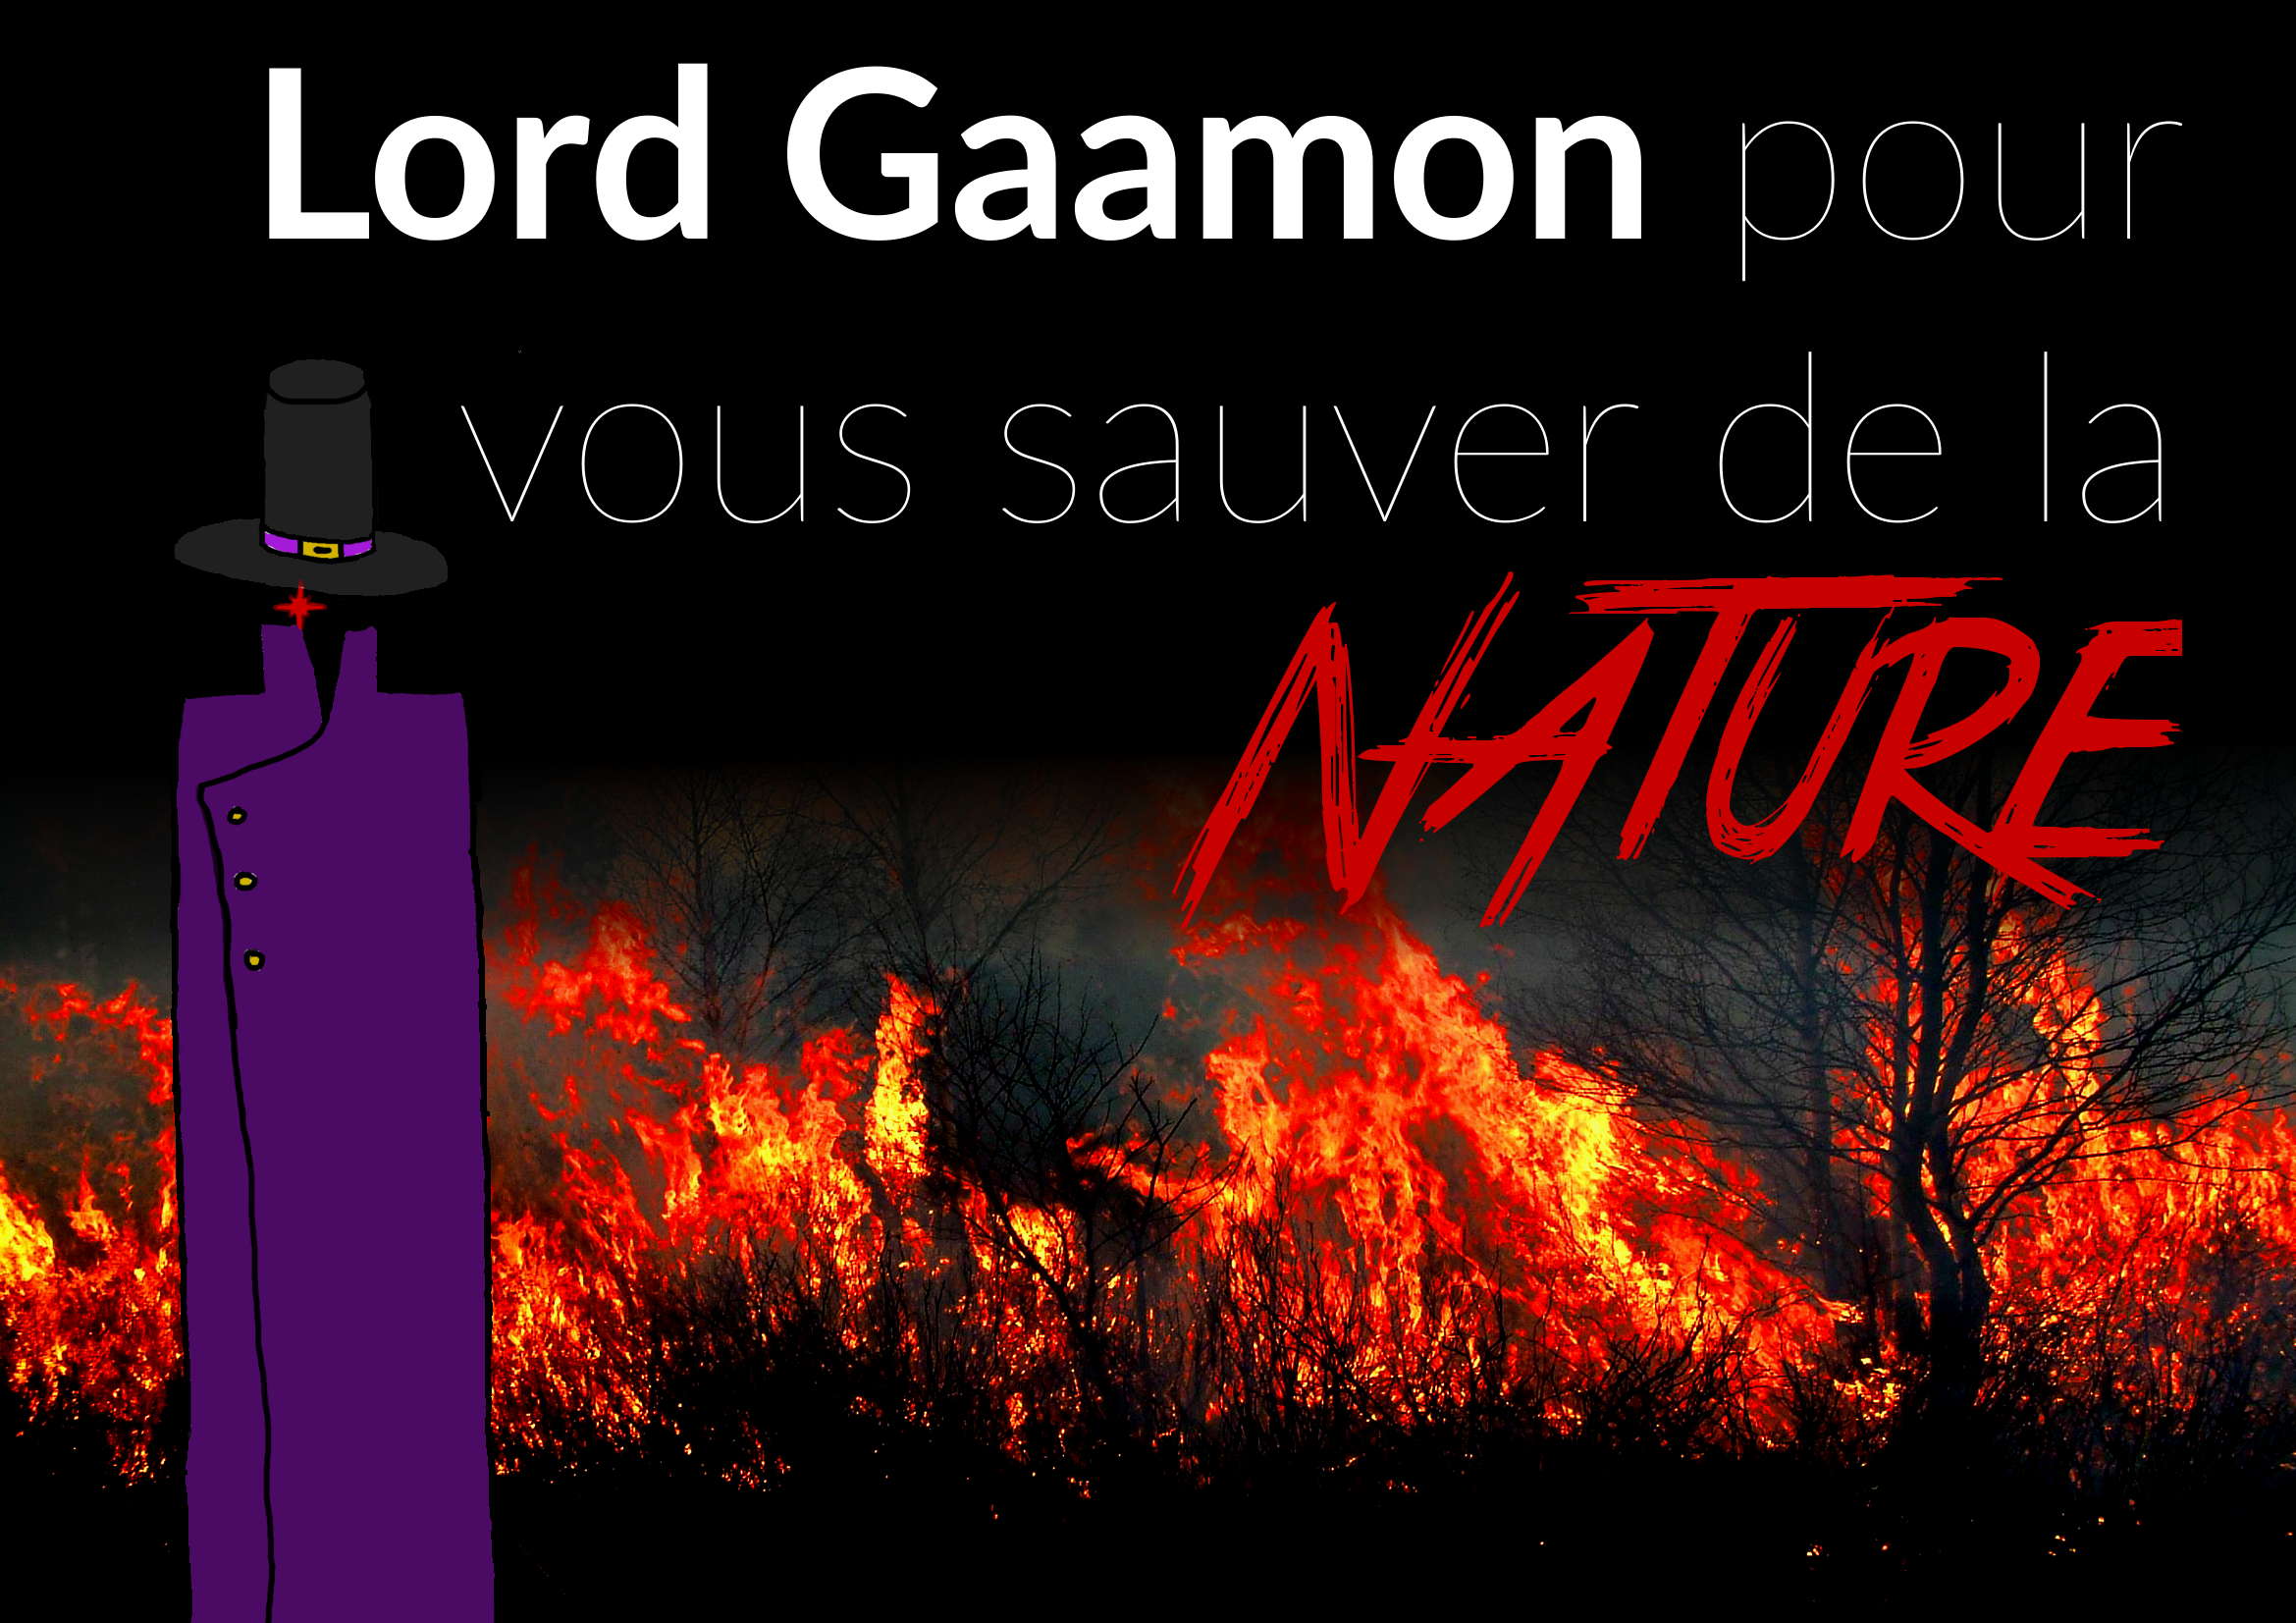
\includegraphics[width=.48\linewidth]{images/Monde/gaamonPourVousSauverNature.png}}
	\hspace*{.04\linewidth}\subfloat[\label{subfig:eliminezTouteNature}Éliminez toute Nature]{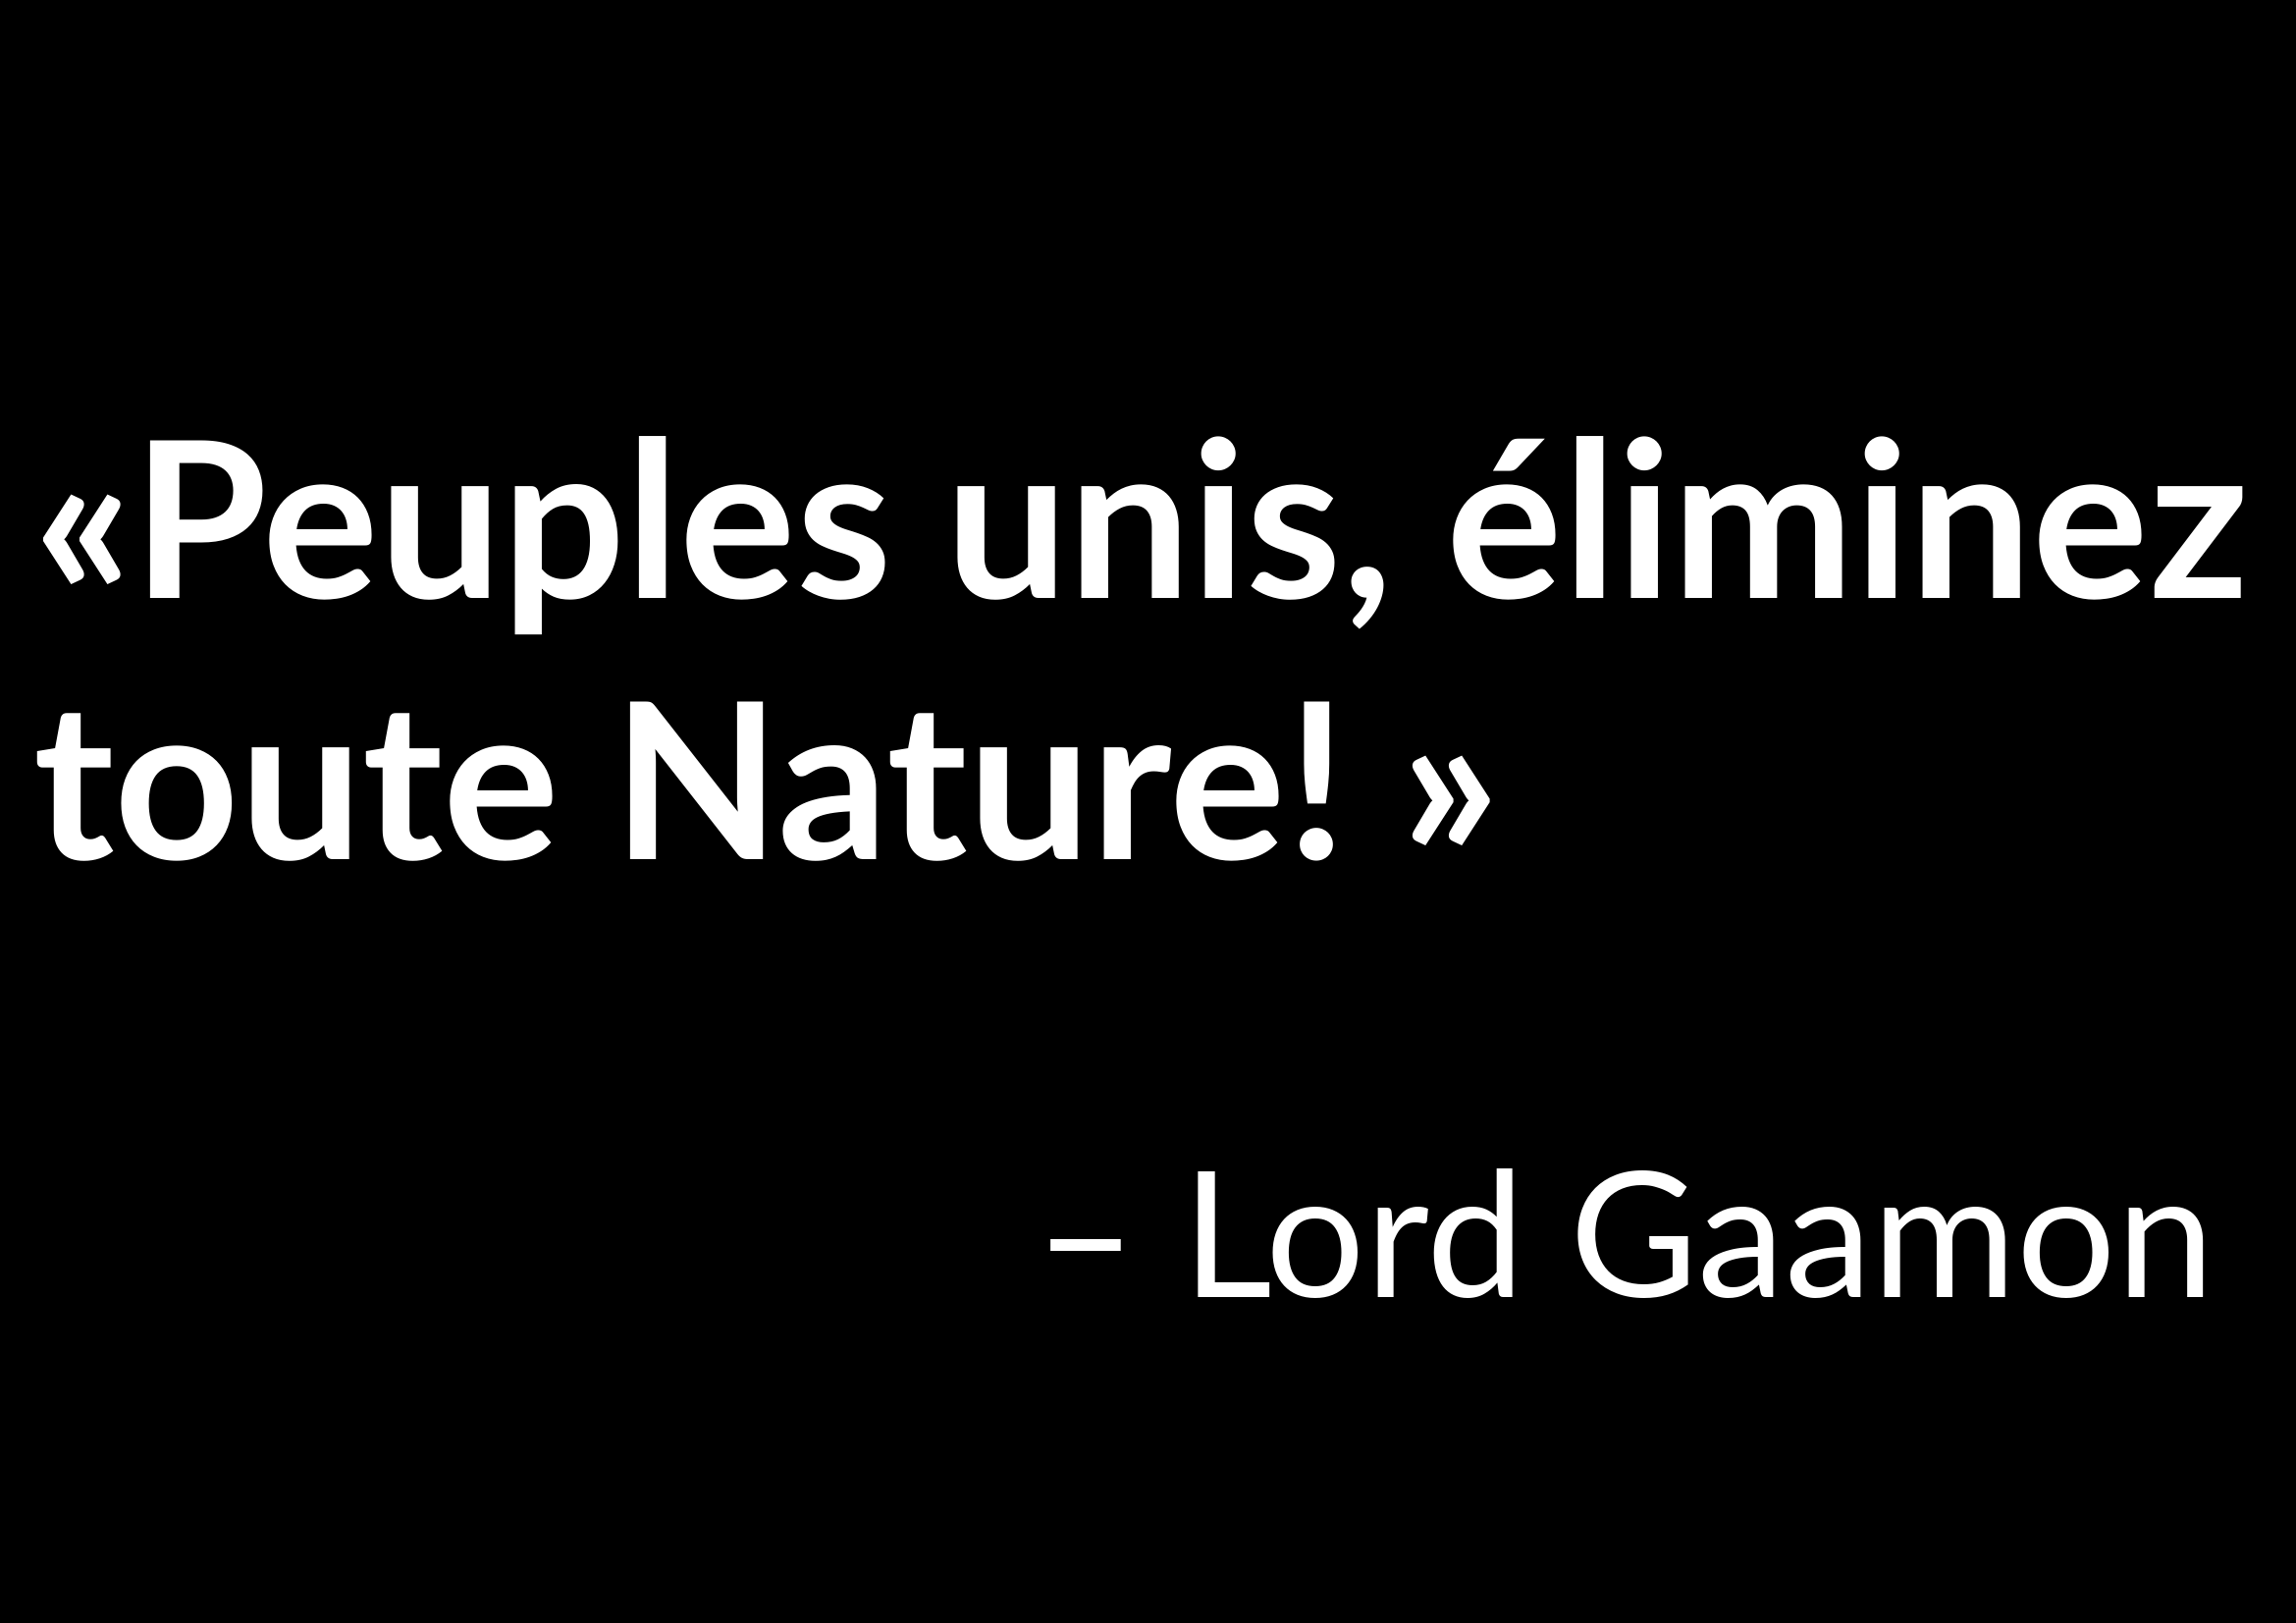
\includegraphics[width=.48\linewidth]{images/Monde/eliminezTouteNature.png}}
	
	\subfloat[\label{subfig:industrialisationPourPuissance}L'industrialisation pour la Puissance]{
\includegraphics[width=.48\textwidth]{images/Monde/industrialisationPourPuissance.png}}
	\hspace*{.04\textwidth}\subfloat[\label{subfig:electricite}Électricité]{
\includegraphics[width=.48\linewidth]{images/Monde/light.png}}
	\caption{\label{fig:propagandeEtatique}Propagande étatique}
\end{figure}



\section{Les \nomNaturels s}

\subsection{Leur histoire}
\label{sec:histoireNaturels}
Les \nomNaturels s étaient, par le passé, le peuple le plus brillant et le plus avancé d'\nomUnivers. Ils avaient trouvé une source d'énergie formidable, l'énergie verte, qui leur permettait de vivre heureux et prospères. L'extraction de cette ressource naturelle était un processus compliqué que seuls les shamans de l'énergie maîtrisaient (\textit{cf.} section \ref{sec:energies}). Grâce à cette source, leurs cités étaient magnifiques, leurs manières connues pour leur raffinement et leur art reconnu pour sa délicatesse.

Ce peuple jouissait d'une prospérité jusque-là sans égale dans l'histoire et répandait sa sagesse, ses connaissances et son amour de la nature de par le monde. L'ascension au pouvoir de Gaamon marqua la fin de cette période; afin d'empêcher la propagation d'un idéal qui mettait la Nature au centre des préoccupations, il fit assassiner les prêtres de l'énergie. Les \nomNaturels s se retrouvèrent subitement privés de leur source vitale --- l'énergie verte --- sans protection et virent leur civilisation s'effondrer brutalement.

Les \nomNaturels s vivent maintenant reclus sur de hauts plateaux, cachés de la haine ainsi que des persécutions de Gaamon et rêvent de leur gloire passée. Si leur idéologie d'amour envers la Nature perdure, leur civilisation décline inexorablement.



\section{Énergies}
\label{sec:energies}
Les énergies sont un élément clé de ce monde. Elles déterminent quels peuples survivront et lesquels disparaîtront. C'est un parallèle de notre dépendance à l'énergie. En effet, on ne peut plus imaginer aujourd'hui vivre sans électricité. À \nomUnivers, les sources d'énergie sont diverses et représentatives des peuples.

\subsection{Humains}
Chez les Humains, l'énergie est tirée du charbon pour créer de la vapeur et de l'électricité. C'est une source très polluante. La couleur qui lui est attribuée est le rouge du feu des hauts fourneaux et le noir de la fumée qui remplit le ciel de \nomVille. Elle fait partie intégrante du Steampunk, caractéristique de ce peuple.

\subsection{\nomNaturels s}
\label{sec:energieTelurans}
À l'inverse, les \nomNaturels s ont exploité l'énergie des arbres, appelée énergie verte. Les plantes fournissaient un apport énergétique et, en contrepartie, les \nomNaturels s portaient une attention toute particulière à leur santé, reproduction, protection et longévité. Une symbiose existait entre les \nomNaturels s et la Nature, un équilibre grandement profitable autant pour l'un que pour l'autre. L'énergie verte était extraite dans la grande salle, dont l'accès était réservé aux grands shamans de l'énergie, seules personnes à pouvoir maîtriser son fonctionnement complexe. Si ce secret était aussi bien gardé, c'est que cette énergie extrêmement puissante, extraite en trop grandes quantités, pouvait causer la mort de milliers d'arbres et animaux. Et un tel cas de figure était à craindre fortement, car la Nature se serait alors retournée contre ceux qui auraient abusé de ses ressources et, dans sa fureur, aurait annihilé des peuples entiers. Les \nomNaturels s, craignant une pareille situation, s'en étaient prémunis en cachant les mécanismes de la grande salle pour ne les révéler qu'aux seuls élus, les shamans.

Cette énergie pouvait également être maîtrisée, dans une moindre mesure, à titre personnel. Les personnes dotées de telles capacités pouvaient alors lancer des \enquote{sorts}. Ceci est un des éléments clé du gameplay (\textit{cf.} section \ref{sec:sorts}). On pourrait comparer l'énergie verte à de la magie mais cela n'est que partiellement correct: l'énergie verte n'est ni illimitée, ni gratuite. L'utiliser de façon disproportionnée signifie tuer toute vie alentour. Et si la Nature est généreuse elle peut aussi refuser de donner son bien, voire punir ceux qui en abusent. Il est également possible de l'extraire de soi-même, mais une fois de plus, la réalisation d'une telle opération est dangereuse car elle peut causer la mort de l'exécutant.

Depuis la disparition mystérieuse des shamans (\textit{cf.} section \ref{sec:histoireNaturels}), les \nomNaturels s ont perdu le secret de l'énergie verte. Ils utilisent donc les énergies hydraulique et éolienne, facilement disponibles dans les montagnes où ils vivent. Elles sont cependant bien moins puissantes que l'énergie verte et ne leur permettent de loin pas les miracles qu'ils pouvaient accomplir avec la première.



\section{Bestiaire}
\label{sec:Bestiaire}

\begin{wrapfigure}[12]{r}{.3\textwidth}
	\vspace*{-.8cm}
	\center
	
\includegraphics[width=.3\textwidth]{images/Monde/Gnobol.png}
	\caption{\label{fig:Gnobol}Gnobol}
\end{wrapfigure}
Du point de vue des genres, le monde d'\nomUnivers\ est un croisement entre la science-fiction et la \anglicisme{Fantasy}, car il est peuplé de créatures féériques et rempli des machines futuristes de Gaamon.

\subsection{Créatures humaines}
\subsubsection{Gnobols}
\label{sec:Gnobols}
Les sbires de Gaamon sont des créatures nommées \textit{Gnobols}. Il existe beaucoup de variantes de la créature \enquote{de base}. Certains pourraient être équipés d'une armure, d'autres d'un arc, d'un fusil, de bombes fumantes ou encore de sifflets d'alarme. Ils sont en revanche tous équipés d'un chapeau duquel une fumée noire s'échappe.

Ces créatures sont en fait des machines inventées par Gaamon et produite à la chaine dans les usines de Murtos. (\textit{cf.} figure \ref{fig:Gnobol})

\subsection{Personnalisation de la Nature}
\label{sec:personnalisationNature}
Dans l'univers d'\nomUnivers, la Nature est personnalisée par trois esprits, chacun représentatif d'un aspect de la Nature. La caractéristique qu'il personnifie définit leur apparence:

\begin{table}[ht!]
	\newlength{\tableLength}
	\setlength{\tableLength}{\textwidth+2.34cm}
	
	\hspace*{-2.34cm}
	\begin{tabu} to \tableLength {l l X X X l}
		\rowfont{\fontspec{Lato Heavy}\selectfont\leavevmode\color{white}}
		\rowcolor{mainColor}
		& Esprit & Description & Mots-clé & Apparence & \\
		& Leo & Il est la destruction renouvelatrice, à la fois créateur et destructeur, de son chaos naît la vie & Massif, sans distinction, abrupt, rapide, mort génératrice de vie & Golem, de pierre et de lave en bas, de pierre et d'eau en haut, avec un duvet de plante sur les épaules & \\
		& Tamund & Il est l'intelligence aveugle, l'évolution lente & Évolution, lent, ciblé, mort des plus faibles & Grand séquoia aveugle & \\
		& Tia & Elle est la vivacité sauvage et profite parfois sans pitié & Sauvage, vif, rapide, profiteur, sans-pitié, survie du plus adapté et mort des plus faibles & Écureuil avec des runes sur le dos & \\
	\end{tabu}
	
	\caption{Les trois esprits et leurs caractéristiques}
\end{table}

\begin{figureWithNotes}[p]
	\center
	\thisfloatpagestyle{empty}
	\captionsetup{format=myformat}
	\hspace*{-3.5cm}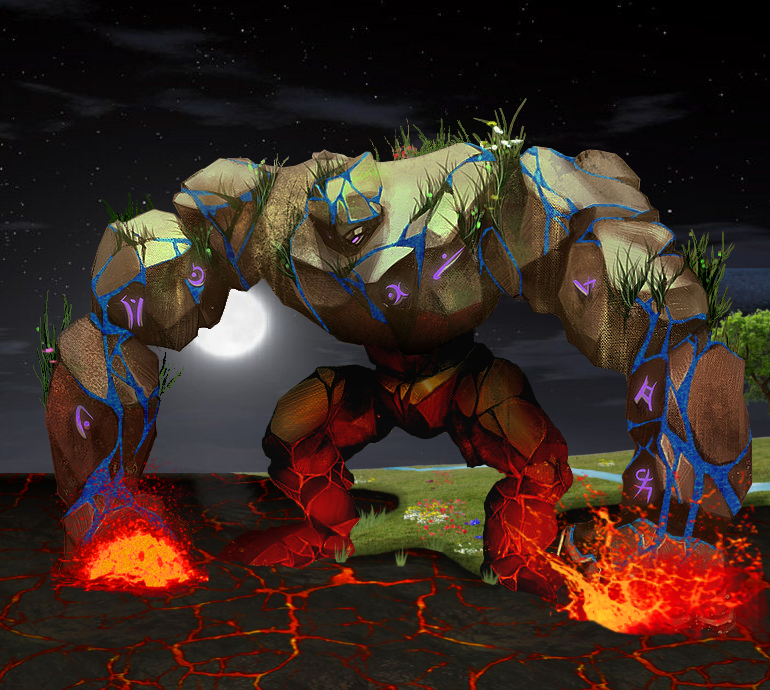
\includegraphics[width=\paperwidth-\myHorizontalTotalMargins]{images/Monde/Leo/Leo.png}
	\caption{Exemple de ce que pourrait être l'apparence de Leo,\\basée sur le travail original de Sinto-risky {\cite{StoneGolem_Sinto-risky}}}
	%\spewnotes
\end{figureWithNotes}
